\documentclass{beamer}
\usepackage[utf8]{inputenc}

\usetheme{Madrid}
\usecolortheme{default}
\usepackage{amsmath,amssymb,amsfonts,amsthm}
\usepackage{txfonts}
\usepackage{tkz-euclide}
\usepackage{listings}
\usepackage{adjustbox}
\usepackage{array}
\usepackage{tabularx}
\usepackage{gvv}
\usepackage{lmodern}
\usepackage{circuitikz}
\usepackage{tikz}
\usepackage{graphicx}

\setbeamertemplate{page number in head/foot}[totalframenumber]

\usepackage{tcolorbox}
\tcbuselibrary{minted,breakable,xparse,skins}



\definecolor{bg}{gray}{0.95}
\DeclareTCBListing{mintedbox}{O{}m!O{}}{%
	breakable=true,
	listing engine=minted,
	listing only,
	minted language=#2,
	minted style=default,
	minted options={%
		linenos,
		gobble=0,
		breaklines=true,
		breakafter=,,
		fontsize=\small,
		numbersep=8pt,
		#1},
	boxsep=0pt,
	left skip=0pt,
	right skip=0pt,
	left=25pt,
	right=0pt,
	top=3pt,
	bottom=3pt,
	arc=5pt,
	leftrule=0pt,
	rightrule=0pt,
	bottomrule=2pt,
	toprule=2pt,
	colback=bg,
	colframe=orange!70,
	enhanced,
	overlay={%
		\begin{tcbclipinterior}
			\fill[orange!20!white] (frame.south west) rectangle ([xshift=20pt]frame.north west);
	\end{tcbclipinterior}},
	#3,
}
\lstset{
	language=C,
	basicstyle=\ttfamily\small,
	keywordstyle=\color{blue},
	stringstyle=\color{orange},
	commentstyle=\color{green!60!black},
	numbers=left,
	numberstyle=\tiny\color{gray},
	breaklines=true,
	showstringspaces=false,
}
%------------------------------------------------------------
%This block of code defines the information to appear in the
%Title page
\title %optional
{1.10.2}
%\subtitle{A short story}

\author % (optional)
{RAVULA SHASHANK REDDY - EE25BTECH11047}

 \begin{document}
	
	
	\frame{\titlepage}
	\begin{frame}{Question}
		Check whether the points \( (7,10),\; (-2,5),\; (3,4) \) form an isosceles right triangle.\\

	\end{frame}
	\begin{frame}{allowframebreaks}
		\frametitle{Equation}
	\textbf{The condition for two sides to be perpendicular : }
		\centering
		
		\label{tab:parameters}
		\begin{align*}
			\vec{n_1^T}\vec{n_2}=0
		\end{align*}
		\end{frame}	
	
	\begin{frame}{Theoretical Solution}
Given:
\begin{align}
\vec{A} = \myvec{7 \\ 10} \\
\vec{B} = \myvec{-2 \\ 5} \\
\vec{C} = \myvec{3 \\ 4}
\end{align}

Side vectors:
\begin{align}
\vec{A}-\vec{B} &= \myvec{7 \\ 10} - \myvec{-2 \\ 5} = \myvec{9 \\ 5} \\
\vec{A}-\vec{C} &= \myvec{7 \\ 10} - \myvec{3 \\ 4} = \myvec{4 \\ 6} \\
\vec{B}-\vec{C} &= \myvec{-2 \\ 5} - \myvec{3 \\ 4} = \myvec{-5 \\ 1}
\end{align}
\end{frame}
\begin{frame}{Theoretical Solution}
Isosceles check:\\

1. Altitude from $\vec{A}$ 
\begin{align}
\vec{D}=\frac{\vec{B}+\vec{C}}{2}
=\frac{1}{2}\myvec{-2+3\\5+4}
=\myvec{\tfrac{1}{2}\\\tfrac{9}{2}}.\\
\vec{A}-\vec{D}
=\myvec{\tfrac{13}{2}\\\tfrac{11}{2}},\qquad
\vec{B}-\vec{C}
=\myvec{-5\\1}.\\
(\vec{A}-\vec{D})^{T}(\vec{B}-\vec{C})
=\myvec{\tfrac{13}{2} & \tfrac{11}{2}}
\myvec{-5\\1}
=-\tfrac{65}{2}+\tfrac{11}{2}\neq 0.
\end{align}


2. Altitude from $\vec{B}$
\begin{align}
\vec{E}=\frac{\vec{C}+\vec{A}}{2}
=\myvec{5\\7}.\\
\vec{B}-\vec{E}=\myvec{-7\\-2},\qquad
\vec{C}-\vec{A}=\myvec{-4\\-6}.
\end{align}
\end{frame}
\begin{frame}{Theoretical Solution}
\begin{align}
(\vec{B}-\vec{E})^{T}(\vec{C}-\vec{A})
=\myvec{-7 & -2}\myvec{-4\\-6}
=28+12=40\neq 0.
\end{align}
 
3.Altitude from $\vec{C}$
\begin{align}
\vec{F}=\frac{\vec{A}+\vec{B}}{2}
=\myvec{\tfrac{5}{2}\\\tfrac{15}{2}}.\\
\vec{C}-\vec{F}=\myvec{\tfrac{1}{2}\\-\tfrac{7}{2}},\qquad
\vec{A}-\vec{B}=\myvec{9\\5}.\\
(\vec{C}-\vec{F})^{T}(\vec{A}-\vec{B})
=\myvec{\tfrac{1}{2} & -\tfrac{7}{2}}
\myvec{9\\5}
=\tfrac{9}{2}-\tfrac{35}{2}=-13\neq0.
\end{align}
\begin{center}    
Hence it is not isosceles triangle.
\end{center}
\end{frame}
\begin{frame}{Theoretical Solution}
Right angle Check:\\

For a right angle, the dot product of two sides must be zero.
\begin{align}
(\vec{A}-\vec{B})^T(\vec{A}-\vec{C}) &= (9)(4) + (5)(6) = 66 \neq 0 \\
(\vec{A}-\vec{B})^T(\vec{B}-\vec{C}) &= (9)(-5) + (5)(1) = -40 \neq 0 \\
(\vec{A}-\vec{C})^T(\vec{B}-\vec{C}) &= (4)(-5) + (6)(1) = -14 \neq 0
\end{align}

Hence, the given points forms neither an isosceles nor a right-angled triangle.
\end{frame}

\begin{frame}[fragile]
		\frametitle{C Code}
		\begin{lstlisting}
    #include <stdio.h>
#include <math.h>

int main() {
    // Coordinates of the points
    int Ax = 7, Ay = 10;
    int Bx = -2, By = 5;
    int Cx = 3, Cy = 4;

    // Squared lengths of sides
    int AB2 = (Ax - Bx) * (Ax - Bx) + (Ay - By) * (Ay - By);
    int AC2 = (Ax - Cx) * (Ax - Cx) + (Ay - Cy) * (Ay - Cy);
    int BC2 = (Bx - Cx) * (Bx - Cx) + (By - Cy) * (By - Cy);

    // Dot products (for right angle check)
    int dot_AB_AC = (Ax - Bx) * (Ax - Cx) + (Ay - By) * (Ay - Cy);
    \end{lstlisting}
    \end{frame}
    \begin{frame}[fragile]
		\frametitle{C Code}
		\begin{lstlisting}
    int dot_AB_BC = (Ax - Bx) * (Bx - Cx) + (Ay - By) * (By - Cy);
    int dot_AC_BC = (Ax - Cx) * (Bx - Cx) + (Ay - Cy) * (By - Cy);

    printf("Squared side lengths:\n");
    printf("AB^2 = %d\n", AB2);
    printf("AC^2 = %d\n", AC2);
    printf("BC^2 = %d\n", BC2);

    printf("\nDot products:\n");
    printf("(A-B)·(A-C) = %d\n", dot_AB_AC);
    printf("(A-B)·(B-C) = %d\n", dot_AB_BC);
    printf("(A-C)·(B-C) = %d\n", dot_AC_BC);
 \end{lstlisting}
    \end{frame}
    \begin{frame}[fragile]
		\frametitle{C Code}
		\begin{lstlisting}
    // Check isosceles right triangle
    if ((AB2 == AC2 && dot_AB_AC == 0) ||
        (AB2 == BC2 && dot_AB_BC == 0) ||
        (AC2 == BC2 && dot_AC_BC == 0)) {
        printf("\nThe points form an ISOSCELES RIGHT triangle.\n");
    } else {
        printf("\nThe points DO NOT form an isosceles right triangle.\n");
    }

    return 0;
}
\end{lstlisting}
\end{frame}
 \begin{frame}[fragile]
		\frametitle{Python Direct Code}
		\begin{lstlisting}
        import numpy as np
import matplotlib.pyplot as plt

# local imports
from libs.line.funcs import line_gen
from libs.triangle.funcs import *

# Coordinates of the points
A = np.array(([7, 10])).reshape(-1, 1)
B = np.array(([-2, 5])).reshape(-1, 1)
C = np.array(([3, 4])).reshape(-1, 1)

# Squared lengths of sides
AB2 = np.sum((A - B) ** 2)
AC2 = np.sum((A - C) ** 2)
BC2 = np.sum((B - C) ** 2)
\end{lstlisting}
\end{frame}
 \begin{frame}[fragile]
		\frametitle{Python Direct Code}
		\begin{lstlisting}
# Dot products
dot_AB_AC = np.dot((A - B).T, (A - C))[0, 0]
dot_AB_BC = np.dot((A - B).T, (B - C))[0, 0]
dot_AC_BC = np.dot((A - C).T, (B - C))[0, 0]

print("Squared side lengths:")
print(f"AB^2 = {AB2}")
print(f"AC^2 = {AC2}")
print(f"BC^2 = {BC2}")

print("\nDot products:")
print(f"(A-B)·(A-C) = {dot_AB_AC}")
print(f"(A-B)·(B-C) = {dot_AB_BC}")
print(f"(A-C)·(B-C) = {dot_AC_BC}")
\end{lstlisting}
\end{frame}
 \begin{frame}[fragile]
		\frametitle{Python Direct Code}
		\begin{lstlisting}
# Check isosceles right triangle
if ((AB2 == AC2 and dot_AB_AC == 0) or
    (AB2 == BC2 and dot_AB_BC == 0) or
    (AC2 == BC2 and dot_AC_BC == 0)):
  
    result = "ISOSCELES RIGHT triangle"
else:
    result = "NOT an isosceles right triangle"

print(f"\nThe points form {result}.")
\end{lstlisting}
\end{frame}
 \begin{frame}[fragile]
		\frametitle{Python Direct Code}
		\begin{lstlisting}
# ---- Plotting ----
x_AB = line_gen(A, B)
x_BC = line_gen(B, C)
x_CA = line_gen(C, A)

plt.plot(x_AB[0, :], x_AB[1, :], 'b')
plt.plot(x_BC[0, :], x_BC[1, :], 'b')
plt.plot(x_CA[0, :], x_CA[1, :], 'b')

# Mark points
tri_coords(A, B, C, ['A(7,10)', 'B(-2,5)', 'C(3,4)'])

# Title
plt.title(f"Triangle ABC: {result}")
plt.gca().set_aspect('equal', adjustable='box')
plt.grid(True)
plt.show()
        \end{lstlisting}
\end{frame}

 \begin{frame}[fragile]
		\frametitle{Python Shared Output}
		\begin{lstlisting}
        import ctypes
import numpy as np
import matplotlib.pyplot as plt

# Define C int type
c_int = ctypes.c_int

def main():
    # Coordinates of the points (numpy arrays)
    A = np.array([c_int(7).value, c_int(10).value])
    B = np.array([c_int(-2).value, c_int(5).value])
    C = np.array([c_int(3).value, c_int(4).value])

    # Squared lengths of sides
    AB2 = c_int(np.sum((A - B) ** 2))
    AC2 = c_int(np.sum((A - C) ** 2))
    BC2 = c_int(np.sum((B - C) ** 2))
  \end{lstlisting}
\end{frame}

 \begin{frame}[fragile]
		\frametitle{Python Shared Output}
		\begin{lstlisting}
    # Dot products (for right angle check)
    dot_AB_AC = c_int(np.dot(A - B, A - C))
    dot_AB_BC = c_int(np.dot(A - B, B - C))
    dot_AC_BC = c_int(np.dot(A - C, B - C))

    print("Squared side lengths:")
    print(f"AB^2 = {AB2.value}")
    print(f"AC^2 = {AC2.value}")
    print(f"BC^2 = {BC2.value}")

    print("\nDot products:")
    print(f"(A-B)·(A-C) = {dot_AB_AC.value}")
    print(f"(A-B)·(B-C) = {dot_AB_BC.value}")
    print(f"(A-C)·(B-C) = {dot_AC_BC.value}")

    # Check isosceles right triangle
    if ((AB2.value == AC2.value and dot_AB_AC.value == 0) or
        (AB2.value == BC2.value and dot_AB_BC.value == 0) or
          \end{lstlisting}
\end{frame}

 \begin{frame}[fragile]
		\frametitle{Python Shared Output}
		\begin{lstlisting}
        (AC2.value == BC2.value and dot_AC_BC.value == 0)):
        result = "ISOSCELES RIGHT triangle"
    else:
        result = "NOT an isosceles right triangle"
    print(f"\nThe points form {result}.")

    # ---- Plotting ----
    fig, ax = plt.subplots()
    # Draw triangle edges
    triangle = np.array([A, B, C, A])  # closed loop
    ax.plot(triangle[:, 0], triangle[:, 1], 'b-o', linewidth=2)

    # Annotate points
    ax.text(A[0]+0.2, A[1]+0.2, "A(7,10)", color="red")
    ax.text(B[0]+0.2, B[1]+0.2, "B(-2,5)", color="red")
    ax.text(C[0]+0.2, C[1]+0.2, "C(3,4)", color="red")
  \end{lstlisting}
\end{frame}

 \begin{frame}[fragile]
		\frametitle{Python Shared Output}
		\begin{lstlisting}
    # Title
    ax.set_title(f"Triangle ABC: {result}")
    ax.set_aspect('equal', adjustable='box')
    ax.grid(True)

    plt.show()

if __name__ == "__main__":
    main()s
        \end{lstlisting}
        \end{frame}
        \begin{frame}{Plot}
        \begin{figure}
            \centering
            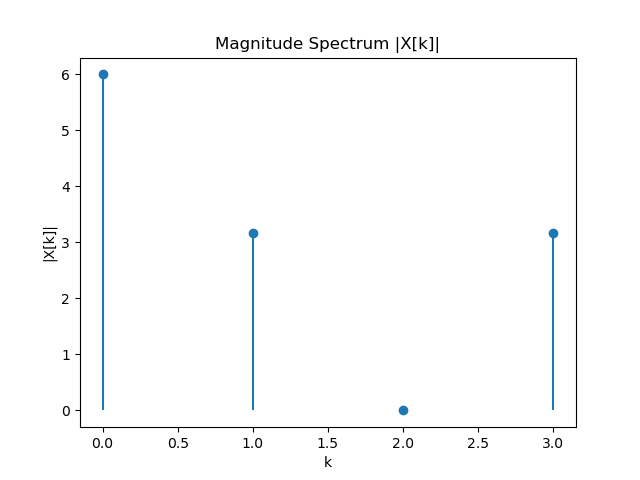
\includegraphics[width=0.9\linewidth]{fig1.png}
            \caption{}
            \label{fig:placeholder}
        \end{figure}
        \end{frame}
\end{document}